% =============================================================================
%  PDS 2026.2 - DESAFIO 08
%  Discretizacao de Filtros IIR por Invariancia ao Impulso e
%  Analise de Aliasing Espectral
%
%  Apresentacao oral - 10 minutos (7-8 min de exposicao + 2-3 min de arguicao)
%
%  Compilar (na pasta slides/):
%      pdflatex -interaction=nonstopmode apresentacao_desafio08.tex
%      pdflatex -interaction=nonstopmode apresentacao_desafio08.tex
%
%  Pacotes necessarios (instalacao minima):
%      tlmgr install beamer pgf translator lmodern booktabs babel-portuguese
%
%  As figuras usadas estao em ../figuras/*.pdf (vetoriais, geradas por
%  src/desafio08.py). Os textos de fala estao em \note{} (modo apresentador).
% =============================================================================
\documentclass[aspectratio=169,10pt]{beamer}

\usepackage[T1]{fontenc}
\usepackage[utf8]{inputenc}
\usepackage[brazilian]{babel}
\usepackage{lmodern}
\usepackage{amsmath,amssymb}
\usepackage{graphicx}
\usepackage{booktabs}
\graphicspath{{../figuras/}}

\usetheme{Madrid}
\usecolortheme{default}
\setbeamertemplate{navigation symbols}{}
\setbeamertemplate{caption}[numbered]

\definecolor{azulPDS}{RGB}{31,78,121}
\definecolor{vermPDS}{RGB}{192,0,0}
\setbeamercolor{structure}{fg=azulPDS}
\setbeamercolor{frametitle}{bg=azulPDS,fg=white}
\setbeamercolor{title}{fg=white,bg=azulPDS}
\setbeamercolor{subtitle}{fg=azulPDS}
\setbeamercolor{author}{fg=black}

% numeros grandes e vermelhos para destacar resultados (funciona em texto e em modo matematico)
\newcommand{\res}[1]{%
  \ifmmode\textcolor{vermPDS}{\boldsymbol{#1}}%
  \else\textcolor{vermPDS}{\textbf{#1}}\fi}

\title[Desafio 08 -- PDS 2026.2]{Desafio 08: Discretização de Filtros IIR por
Invariância ao Impulso e Análise de Aliasing Espectral}
\subtitle{Avaliação em duplas -- 10 minutos}
\author[]{Dupla: {Matheus Sousa} e {Fernanda Lopes}}
\institute{UFPE -- Departamento de Eletrônica e Sistemas (DES)}
\date{PDS 2026.2}

\begin{document}

% ---------------------------------------------------------------- slide 1
\begin{frame}
  \titlepage
  \vspace{-1.0em}
  \begin{center}
    \small $F_s = 40$ kHz ($T_s = 25\,\mu$s) \quad$\bullet$\quad
    $f_0 = 6$ kHz \quad$\bullet$\quad $Q = 60$
  \end{center}
  \note{Boa tarde. Nosso desafio foi projetar um filtro digital passa-faixa por
  invariância ao impulso a partir do protótipo analógico dado, analisar o
  aliasing espectral com Fs = 40 kHz e responder por que o método falha no
  passa-altas. Códigos, figuras e verificações ficam à disposição. (15 s)}
\end{frame}

% ---------------------------------------------------------------- slide 2
\begin{frame}{Contexto e protótipo analógico}
  \begin{block}{Enunciado: protótipo passa-faixa de 2ª ordem}
    \[
      H_a(s)=\frac{s}{s^2+200\pi s+(12000\pi)^2}
             =\frac{s}{s^2+2\zeta\omega_n s+\omega_n^2}
    \]
  \end{block}
  \begin{itemize}
    \item $\omega_n = 12000\pi = 37\,699{,}1118$ rad/s \quad($f_n = 6$ kHz)
    \item $2\zeta\omega_n = 200\pi \Rightarrow \zeta = 1/120 = 8{,}333\times10^{-3}
          \Rightarrow \res{Q = 60}$ (filtro seletivo)
    \item $\sigma = \zeta\omega_n = 100\pi$ rad/s \quad ; \quad
          $\omega_d = 100\pi\sqrt{14399} = 37\,697{,}8028$ rad/s
    \item Método exigido: \textbf{invariância ao impulso} com $T_s = 25\,\mu$s
    \item Definição: $\res{h[n]=T_s\,h_a(nT_s)}$
  \end{itemize}
  \note{Comparando Ha(s) com a forma padrão, o termo de 1ª ordem dá 2ζωn = 200π,
  logo ζ = 1/120 e Q = 60: filtro muito seletivo. O método amostra a resposta ao
  impulso e depois calculamos H(z) = Σ h[n] z⁻ⁿ. (40 s)}
\end{frame}

% ---------------------------------------------------------------- slide 3
\begin{frame}{Item 1 -- resposta ao impulso analógica $h_a(t)$}
  \begin{columns}[T]
    \begin{column}{0.48\textwidth}
      \small
      \textbf{Frações parciais:}
      \[
        \frac{s}{(s+\sigma)^2+\omega_d^2}
        =\frac{s+\sigma}{(s+\sigma)^2+\omega_d^2}
        -\frac{\sigma}{(s+\sigma)^2+\omega_d^2}
      \]
      \textbf{Resultado (tabelas de Laplace):}
      \[
        h_a(t)=e^{-100\pi t}\!\left[\cos(\omega_d t)
        -\frac{1}{\sqrt{14399}}\sin(\omega_d t)\right]\!u(t)
      \]
    \end{column}
    \begin{column}{0.48\textwidth}
      \begin{itemize}
        \item $\omega_d = 100\pi\sqrt{14399} = 37\,697{,}8028$ rad/s \\
              ($f_d = 5999{,}79$ Hz)
        \item $h_a(0^+)=1$ e $h_a(0^-)=0$: há um \textbf{salto em $t=0$}
        \item $|H_a(j\omega_n)| = \dfrac{1}{2\zeta\omega_n}
              = \dfrac{1}{200\pi} = 1{,}59155\times10^{-3}$
        \item Forma exata (SymPy): $\bigl(-\tfrac{\sqrt{119}}{1309}
              \sin(1100\sqrt{119}\,\pi t)+\cos(1100\sqrt{119}\,\pi t)\bigr)
              e^{-100\pi t}$
      \end{itemize}
    \end{column}
  \end{columns}
  \note{Decompomos em frações parciais e voltamos pelas tabelas de Laplace.
  Dois pontos de atenção: ωd = 100π√14399 (não ωn — o amortecimento desloca a
  oscilação) e ha(0+) = 1, o salto em t = 0, que reaparece na discussão de
  aliasing. Verificado simbolicamente no SymPy a 1e-16. (40 s)}
\end{frame}

% ---------------------------------------------------------------- slide 4
\begin{frame}{Item 1 -- $h_a(t)$ e as amostras $h[n]/T_s = h_a(nT_s)$}
  \begin{center}
    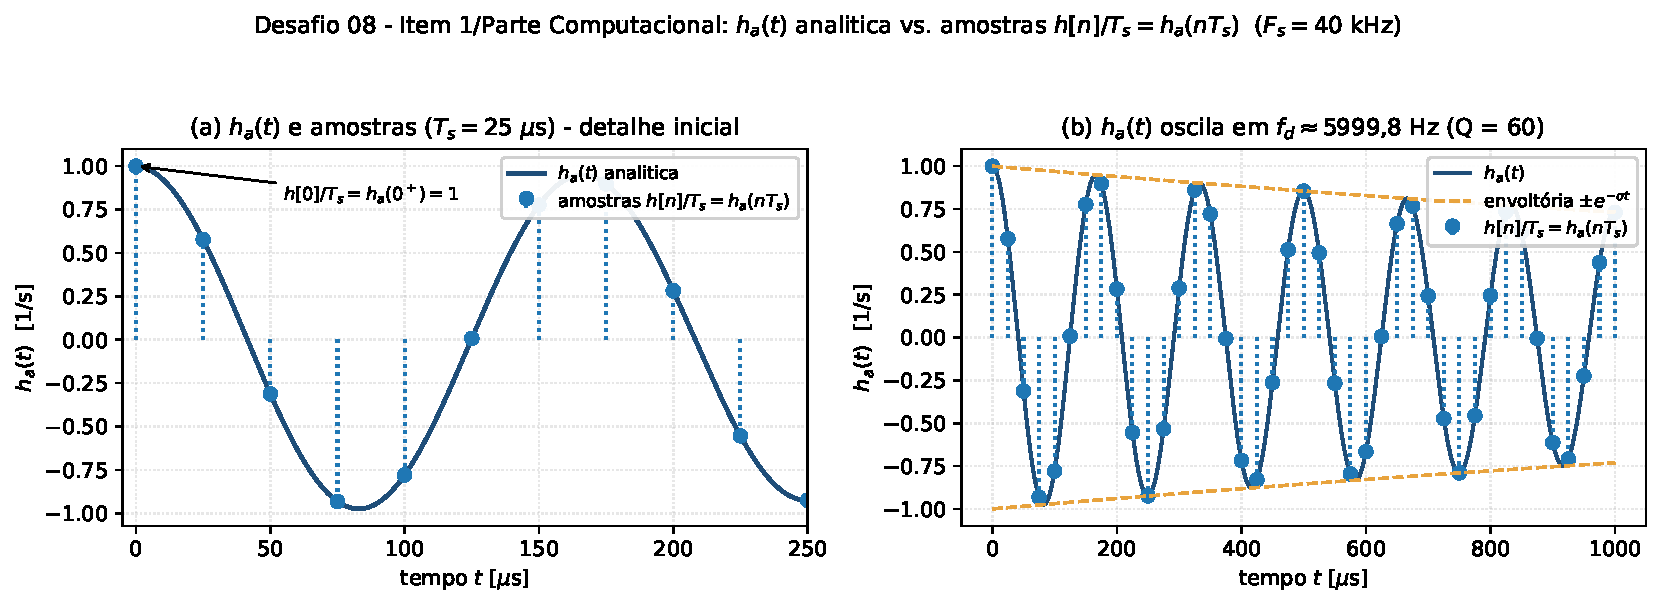
\includegraphics[width=0.95\linewidth]{fig01_ha_t_e_amostras.pdf}
  \end{center}
  \vspace{-0.4em}
  \footnotesize As hastes caem \textbf{exatamente sobre a curva analítica}: é a
  própria definição do método (não há aproximação no domínio do tempo).
  Envoltória $e^{-\sigma t}$ com $\tau = 1/\sigma = 3{,}18$ ms.
  \note{Este gráfico é a definição do método: as hastes são ha(nTs) e caem sobre
  a curva. O filtro tem memória longa porque Q = 60. (20 s)}
\end{frame}

% ---------------------------------------------------------------- slide 5
\begin{frame}{Item 2 -- coeficientes exatos de $H(z)$ (2ª ordem)}
  \small
  Com $r = e^{-\sigma T_s}$ e $\theta = \omega_d T_s$:
  \[
    H(z)=\frac{T_s\left[1-r\left(\cos\theta+\frac{\sigma}{\omega_d}\sin\theta
    \right)z^{-1}\right]}{1-2r\cos\theta\,z^{-1}+r^2z^{-2}}
  \]
  \[
    r = e^{-100\pi\cdot25\mu} = 0{,}992176780 \qquad
    \theta = 0{,}942445070\ \text{rad} = 0{,}29998958\,\pi\ \text{rad/amostra}
  \]
  \begin{block}{Coeficientes numéricos}
    \[
      b_0 = T_s = \res{2{,}500000000\times10^{-5}} \qquad
      b_1 = \res{-1{,}474755715\times10^{-5}}
    \]
    \[
      a_1 = \res{-1{,}166426294} \qquad
      a_2 = \res{0{,}9844147634}
    \]
  \end{block}
  \begin{itemize}
    \item Polos: $z = 0{,}992176780\,e^{\pm j0{,}29999\pi} \Rightarrow |z|<1$
          (\textbf{estável}); zero do método em $z = 0{,}58990$
    \item Ganho em DC: $|H(e^{j0})| = 1{,}2534\times10^{-5} \approx T_s/2$
          (não é exatamente zero -- ver slide 12)
  \end{itemize}
  \note{Escrito com r = exp(-σTs) e θ = ωdTs. Leia os quatro coeficientes
  devagar: b0 = 2,5e-5, b1 = -1,4747557e-5, a1 = -1,166426294,
  a2 = 0,9844147634. Polos em 0,99217678·e^{±j0,29999π}: módulo menor que 1,
  estável; o ângulo corresponde a 5999,79 Hz. O método inventa um zero em
  0,58990 — zeros não mapeiam. Conferido por dois caminhos independentes.
  (50 s)}
\end{frame}

% ---------------------------------------------------------------- slide 6
\begin{frame}{Item 2 -- polos e zeros no plano $z$}
  \begin{center}
    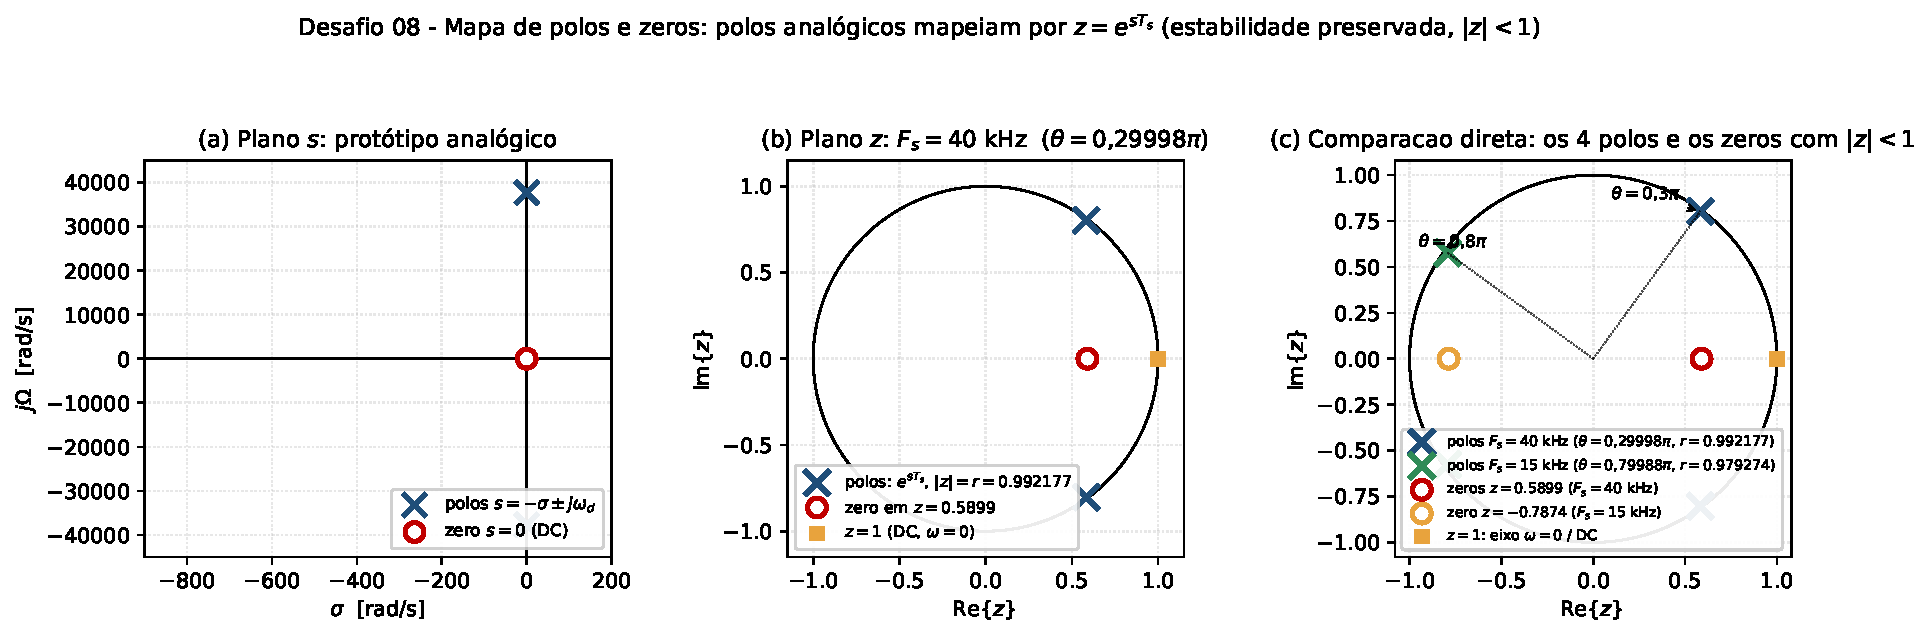
\includegraphics[width=0.98\linewidth]{fig05_polos_zeros.pdf}
  \end{center}
  \vspace{-0.4em}
  \footnotesize Polos analógicos mapeiam por $\res{z=e^{sT_s}}$: raio
  $r = e^{-\sigma T_s}<1$ garante estabilidade. Os \textbf{zeros não são
  mapeados} -- o zero em $s=0$ não vira zero em $z=1$.
  \note{Os polos vão para o plano z por z = e^{sTs}; como o raio é menor que 1,
  a estabilidade é preservada. À direita comparo com Fs = 15 kHz: o polo gira
  para 0,8π, mais perto de Nyquist. E não existe zero em z = 1. (25 s)}
\end{frame}

% ---------------------------------------------------------------- slide 7
\begin{frame}{Item 3 -- ganho de pico em $\omega_0 = 2\pi\cdot6000\cdot T_s = 0{,}3\pi$}
  \begin{center}
    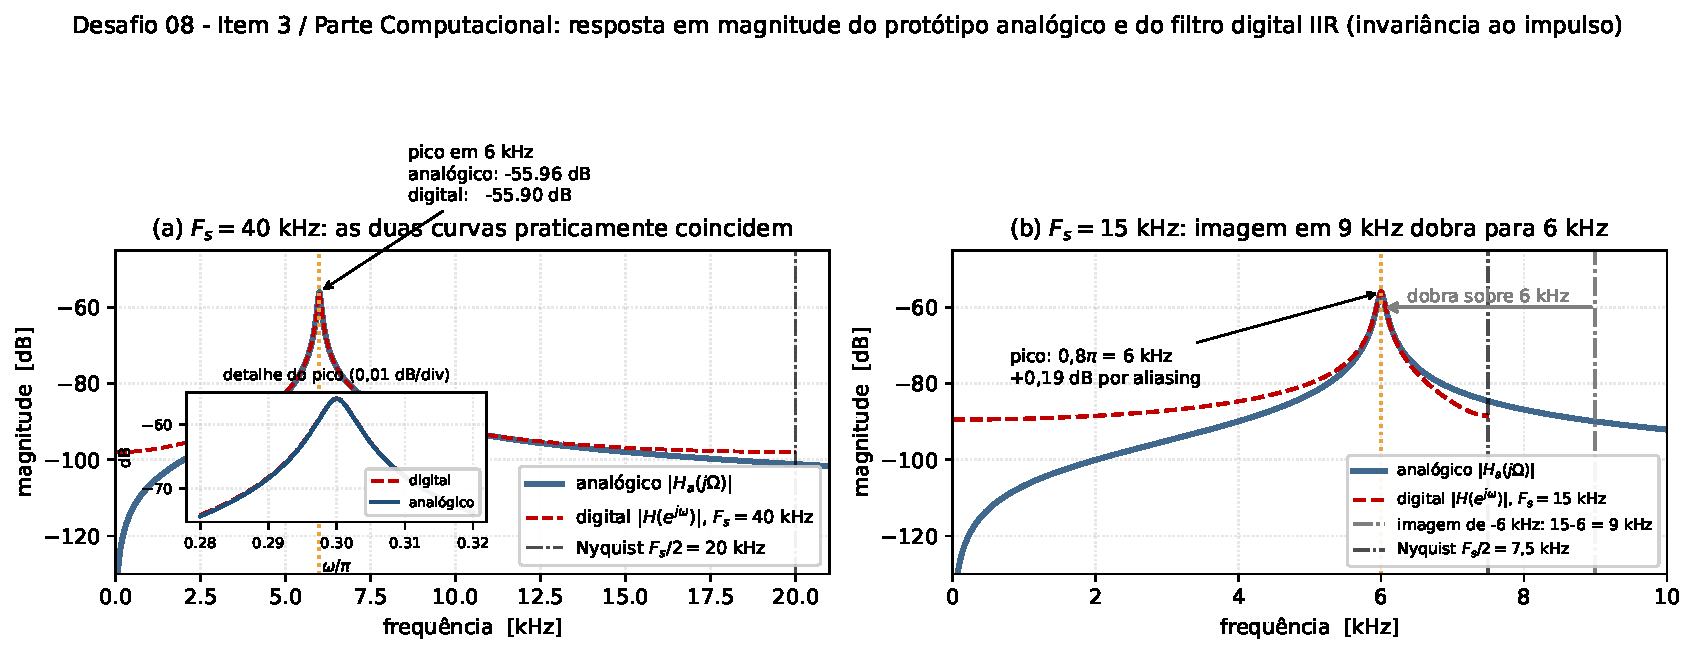
\includegraphics[width=0.99\linewidth]{fig03_magnitude_analogico_vs_digital.pdf}
  \end{center}
  \vspace{-0.5em}
  \footnotesize
  analógico: $|H_a(j\omega_n)| = 1{,}59155\times10^{-3}$ ($-55{,}9636$ dB)
  \quad$\bullet$\quad
  digital: $|H(e^{j0{,}3\pi})| = \res{1{,}60409\times10^{-3}}$ ($-55{,}8954$ dB)
  \quad$\bullet$\quad
  diferença: $\res{+0{,}0685\ \text{dB}}$ ($+0{,}8\,\%$)
  \note{ω0 = 0,3π rad/amostra é exatamente a ressonância, porque ωnTs = 0,3π.
  O ganho analítico é 1/(2ζωn) = 1/(200π). O digital dá 1,60409e-3: diferença de
  +0,0685 dB — NÃO houve alteração significativa. O zoom mostra as duas curvas
  praticamente coincidentes. (40 s)}
\end{frame}

% ---------------------------------------------------------------- slide 8
\begin{frame}{Mecanismo do aliasing: réplicas deslocadas de $kF_s$}
  \begin{center}
    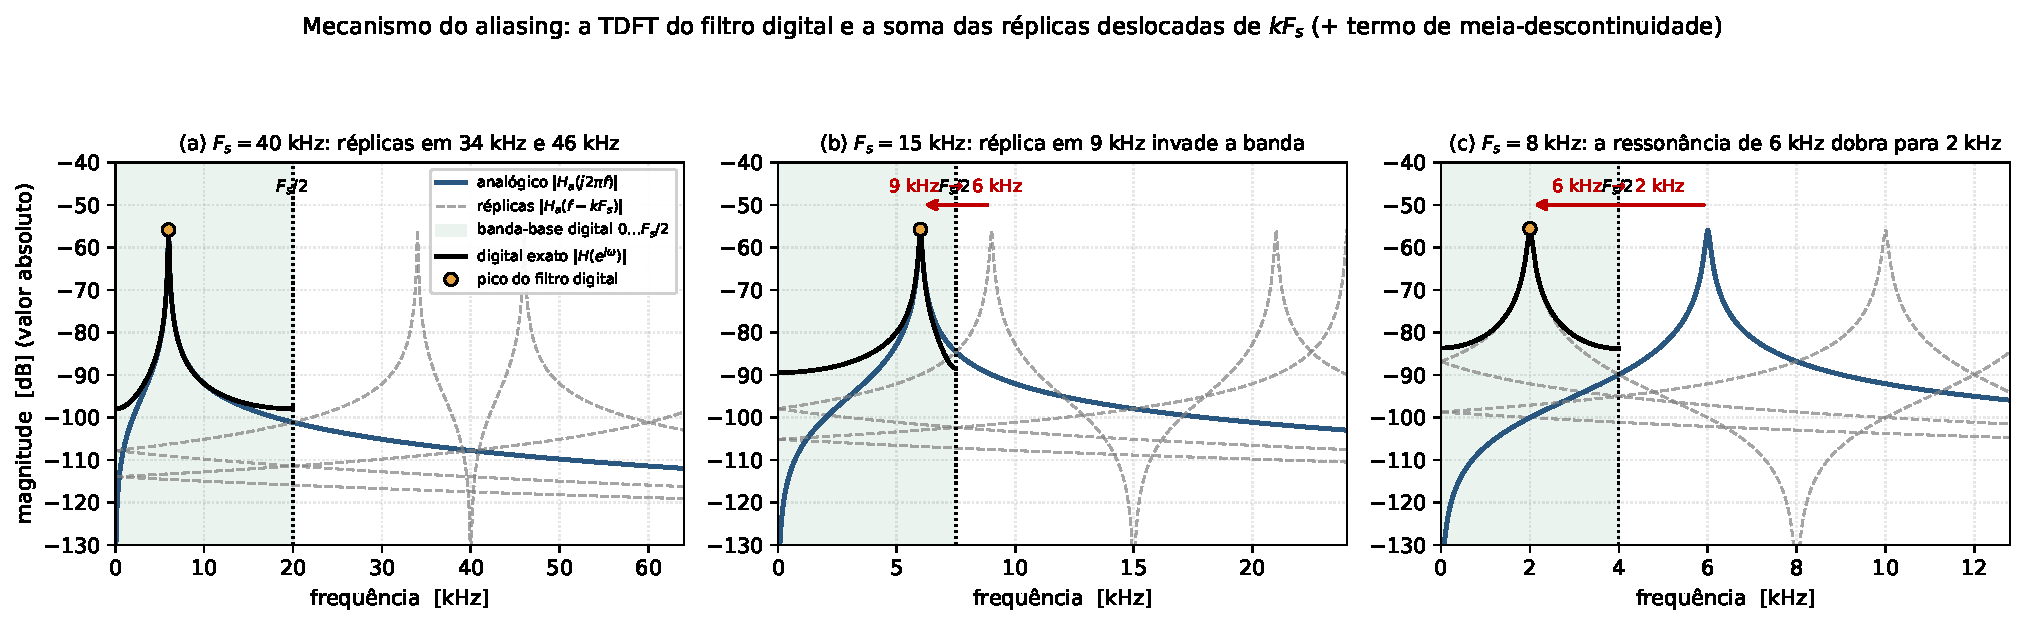
\includegraphics[width=\linewidth]{fig04_aliasing_replicas.pdf}
  \end{center}
  \vspace{-0.6em}
  \footnotesize A TDFT do filtro digital é a soma das réplicas de $H_a$
  deslocadas de $kF_s$: 40 kHz $\Rightarrow$ réplicas em 34/46 kHz;
  15 kHz $\Rightarrow$ imagem em 9 kHz \textbf{dobra para 6 kHz} (+0,19 dB);
  8 kHz $\Rightarrow$ a ressonância inteira dobra para 2 kHz.
  \note{Painel (a): em 40 kHz as réplicas caem em 34 e 46 kHz, longe da
  banda-base. Em 15 kHz a imagem da componente de -6 kHz cai em 9 kHz, que é
  acima de Nyquist (7,5 kHz) e dobra de volta para 6 kHz: +0,19 dB. Em 8 kHz é a
  própria ressonância que fica acima de Nyquist e reaparece em 2 kHz. (35 s)}
\end{frame}

% ---------------------------------------------------------------- slide 9
\begin{frame}{Item 3 -- quando o aliasing passa a importar}
  \begin{center}
    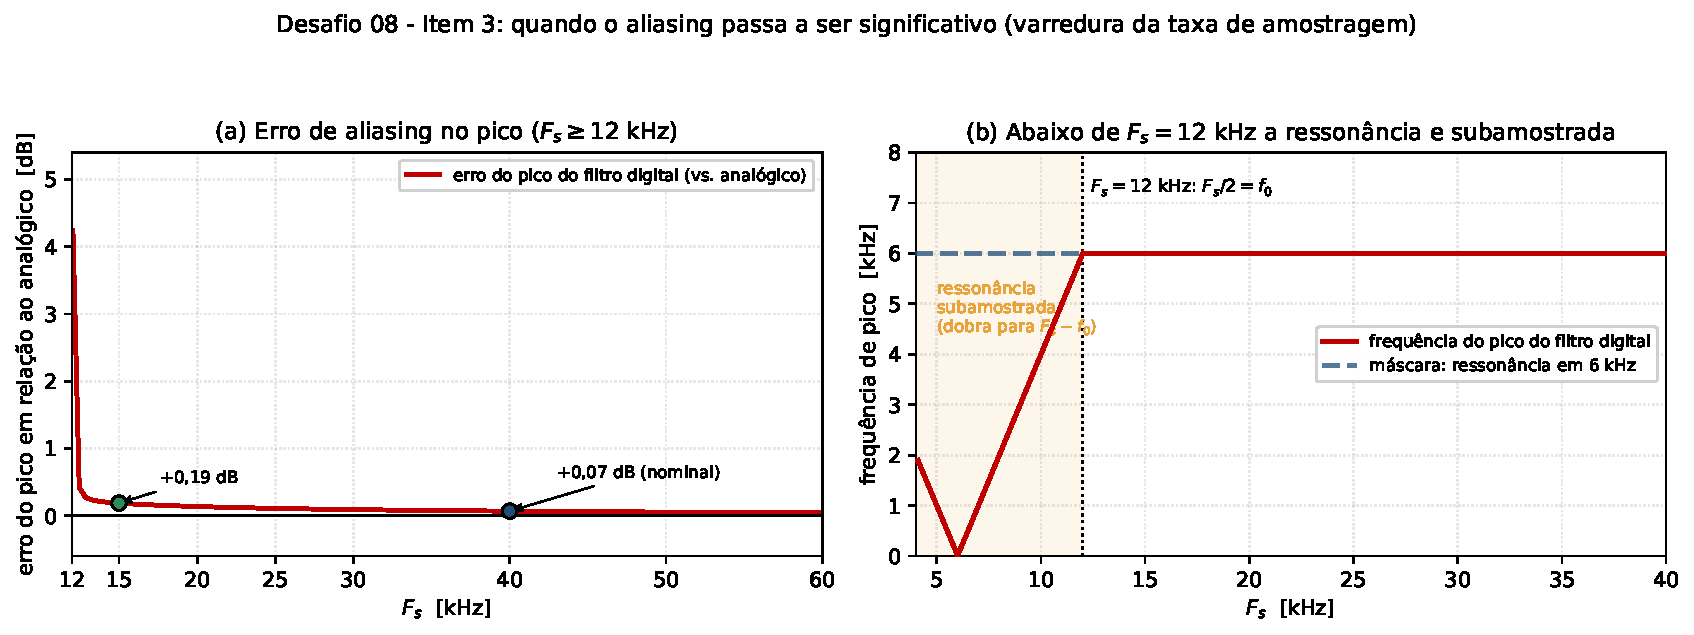
\includegraphics[width=0.99\linewidth]{fig07_erro_aliasing_vs_Fs.pdf}
  \end{center}
  \vspace{-0.5em}
  \footnotesize 40 kHz: $+0{,}07$ dB (nominal) $\bullet$ 15 kHz: $+0{,}19$ dB
  $\bullet$ \res{12 kHz: $+6{,}1$ dB} $\bullet$ abaixo de 12 kHz a ressonância
  de 6 kHz é subamostrada e reaparece em $F_s-6$ kHz.
  \note{Varremos Fs de 12 a 60 kHz. O caso crítico é Fs = 2f0 = 12 kHz, onde a
  ressonância cai exatamente em Nyquist e a imagem se soma em fase: o pico
  DOBRA (medimos 2,026×, +6,1 dB). Abaixo disso, a ressonância é subamostrada —
  em 8 kHz aparece um pico em 2 kHz. (30 s)}
\end{frame}

% --------------------------------------------------------------- slide 10
\begin{frame}{Desafio de reflexão -- o passa-altas degenerado}
  \begin{center}
    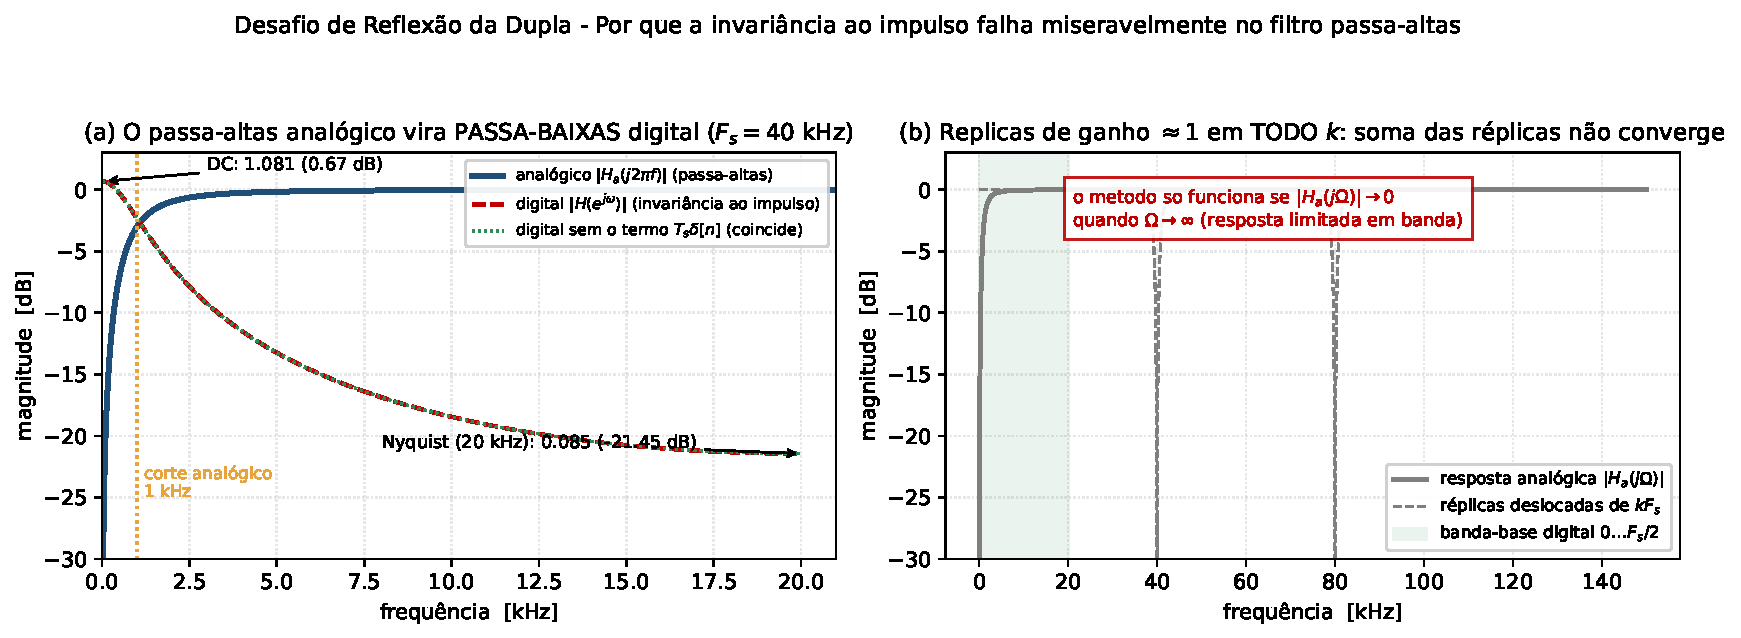
\includegraphics[width=0.99\linewidth]{fig06_falha_passa_altas.pdf}
  \end{center}
  \vspace{-0.5em}
  \footnotesize $H_a(s)=\dfrac{s}{s+2000\pi}$ $\Rightarrow$
  $|H(1)| = \res{1{,}0806}$ ($+0{,}67$ dB) e $|H(-1)| = \res{0{,}0847}$
  ($-21{,}45$ dB): o ganho \textbf{decresce} com a frequência.
  \note{Aplicando o mesmo método ao passa-altas: ha(t) = δ(t) − 2000π e^{...}u(t)
  e o H(z) resultante tem ganho 1,0806 em DC e 0,0847 em Nyquist. O passa-altas
  virou um passa-baixas. E o zero ficou em z ≈ -1,4e-4, praticamente na origem:
  não há zero em z = 1. (45 s)}
\end{frame}

% --------------------------------------------------------------- slide 11
\begin{frame}{Desafio de reflexão -- a explicação matemática}
  \begin{itemize}
    \item Identidade exata do método (soma de Poisson):
      \[
        H(e^{j\omega})=\sum_k H_a\!\left(j\frac{\omega-2\pi k}{T_s}\right)
        +\frac{T_s\,h_a(0^+)}{2}
      \]
    \item No passa-altas $|H_a(j\Omega)|\to 1$ quando $\Omega\to\infty$:
      \textbf{cada réplica vale $\approx 1$} e a série \res{não converge} --
      energia de todo o eixo $\Omega$ é dobrada para dentro da banda digital.
    \item Nenhum $F_s$ corrige: a limitação é do \textbf{método}.
    \item O zero em $s=0$ \textbf{não} é transportado para $z=1$: na invariância
      ao impulso só os \textbf{polos} mapeiam, por $z=e^{sT_s}$.
    \item Consequência: $T_s\,\delta[n]$ (de $\delta(t)$) somado ao passa-baixas
      do polo produz a curva decrescente observada.
    \item Para passa-altas usa-se \textbf{transformação bilinear com
      pré-deformação} (método do Desafio 09).
  \end{itemize}
  \note{A causa é estrutural: no passa-baixas |Ha| → 0 em HF e a soma converge;
  no passa-altas cada réplica vale 1 e a série diverge. Não existe Fs que
  resolva. Algebricamente, o que definia o passa-altas era o zero em s = 0, e
  zeros não mapeiam. A solução é a bilinear com pré-deformação. (45 s)}
\end{frame}

% --------------------------------------------------------------- slide 12
\begin{frame}{Rigor extra e verificação numérica}
  \begin{itemize}
    \item Como $h_a(0^+)=1$, a soma clássica de réplicas fica exatamente
      $T_s/2$ abaixo da resposta exata:
      \[
        \text{medido } \res{1{,}2500\times10^{-5}} \quad\text{vs. previsto}\quad
        \res{1{,}2500\times10^{-5}}
      \]
      Erro relativo final da identidade: $6{,}5\times10^{-5}$.
    \item Isso explica o ganho em DC $\approx T_s/2 = 1{,}2534\times10^{-5}$.
    \item \textbf{23 verificações independentes} (\texttt{src/verificacao.py}):
      \begin{itemize}
        \item $H(z)$ por três caminhos: fórmula fechada, resíduos complexos dos
          polos e TDFT/FFT de $h[n]$ (2$\times$10$^6$ amostras);
        \item polos digitais $=e^{p_aT_s}$; $|z|<1$; $\sum h[n]\approx 0$;
        \item dobramento em 9 kHz $\to$ 6 kHz e pico dobrando em $F_s=12$ kHz.
      \end{itemize}
  \end{itemize}
  \note{Um detalhe que só aparece na conta fina: como ha(0+) = 1, a soma clássica
  de réplicas fica exatamente Ts/2 abaixo da resposta exata — medimos 1,2500e-5
  contra 1,2500e-5. Isso explica o ganho em DC ≈ Ts/2. E rodamos 23 verificações
  independentes: o comando é python src/verificacao.py, sai 23/23. (25 s)}
\end{frame}

% --------------------------------------------------------------- slide 13
\begin{frame}{Resposta ao impulso do filtro digital}
  \begin{center}
    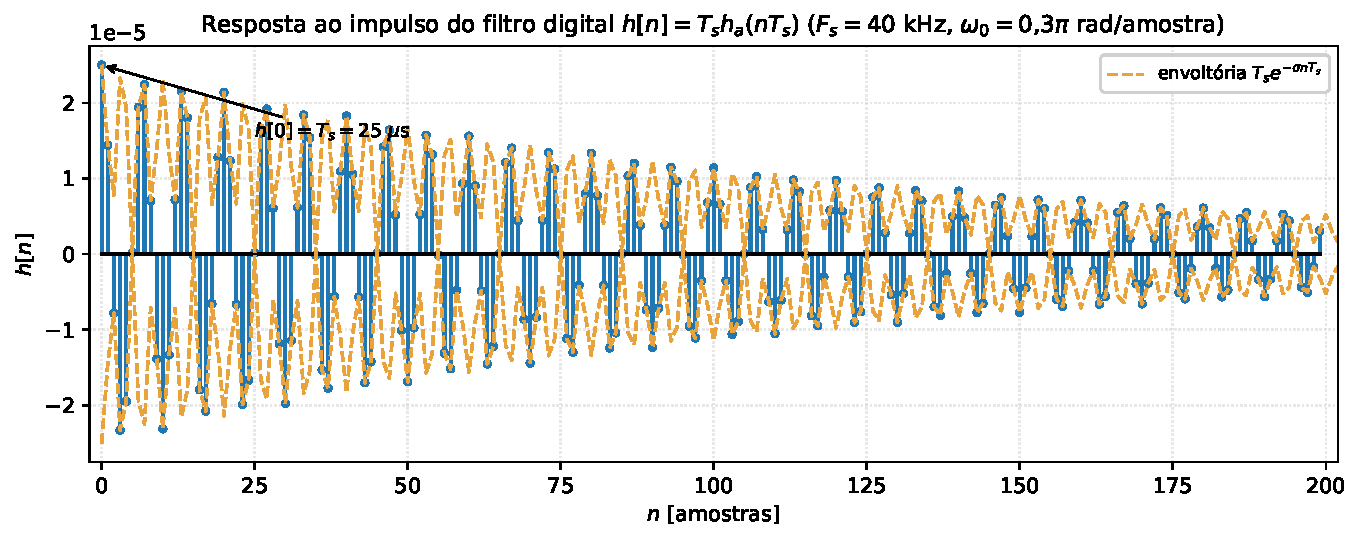
\includegraphics[width=0.92\linewidth]{fig02_resposta_impulso_digital.pdf}
  \end{center}
  \vspace{-0.6em}
  \footnotesize $h[n]$ decai lentamente porque os polos estão a
  $r = 0{,}9922$ do círculo unitário: banda de $-3$ dB de
  $\approx 100$ Hz $\approx f_0/Q$.
  \note{Slide cortável: a resposta ao impulso do filtro digital decai devagar
  porque os polos estão a 0,9922 do círculo unitário; a banda de -3 dB é de
  100 Hz, coerente com f0/Q. (15 s)}
\end{frame}

% --------------------------------------------------------------- slide 14
\begin{frame}{Conclusões}
  \begin{enumerate}
    \item Resolvemos os três itens de forma fechada e verificada: $h_a(t)$, os
      quatro coeficientes de $H(z)$ e o ganho de pico.
    \item O filtro digital é \textbf{estável} ($r = 0{,}9922 < 1$) e de
      \textbf{2ª ordem}, com pico exatamente em $0{,}3\pi$.
    \item Em $F_s = 40$ kHz o pico difere do analógico em \res{+0,07 dB}:
      \textbf{não houve alteração significativa}.
    \item O aliasing é governado por $F_s/2f_0$: 15 kHz custa 0,19 dB,
      \res{12 kHz dobra o pico} e abaixo disso a ressonância é subamostrada.
    \item Ponto principal: a invariância ao impulso \textbf{degenera no
      passa-altas} porque as réplicas não decaem -- a identidade de Poisson
      deixa de convergir.
  \end{enumerate}
  \vspace{0.6em}
  \begin{center}
    \textbf{Obrigado! Perguntas?}
  \end{center}
  \note{Recapitulando os cinco pontos numerados e agradeço. Se o tempo
  apertou, o slide 13 já foi cortado. (35 s)}
\end{frame}

\end{document}
